\documentclass[spanish,12pt,a4paper,titlepage]{report}
\usepackage[utf8]{inputenc}
\usepackage{graphicx}
\usepackage{subfig}
\usepackage{float}
\usepackage{wrapfig}
\usepackage{multirow}
\usepackage{caption}
\usepackage[spanish]{babel}
\usepackage[dvips]{hyperref}
\usepackage{amssymb}
\usepackage{listings}
\usepackage{epsfig}
\usepackage{amsmath}
\usepackage{array}
\usepackage[table]{xcolor}
\usepackage{multirow}
%\usepackage[Sonny]{fncychap}
\usepackage[Lenny]{fncychap}
%\usepackage[Glenn]{fncychap}
%\usepackage[Conny]{fncychap}
%\usepackage[Rejne]{fncychap}
%\usepackage[Bjarne]{fncychap}
%\usepackage[Bjornstrup]{fncychap}

%\usepackage{subfiles}
%\usepackage{framed}

\setlength{\topmargin}{-1.5cm}
\setlength{\textheight}{25cm}
\setlength{\oddsidemargin}{0.3cm} 
\setlength{\textwidth}{15cm}
\setlength{\columnsep}{0cm}

\begin{document}

\chapter{División de tareas}

\begin{figure}[h!]
	\centering
	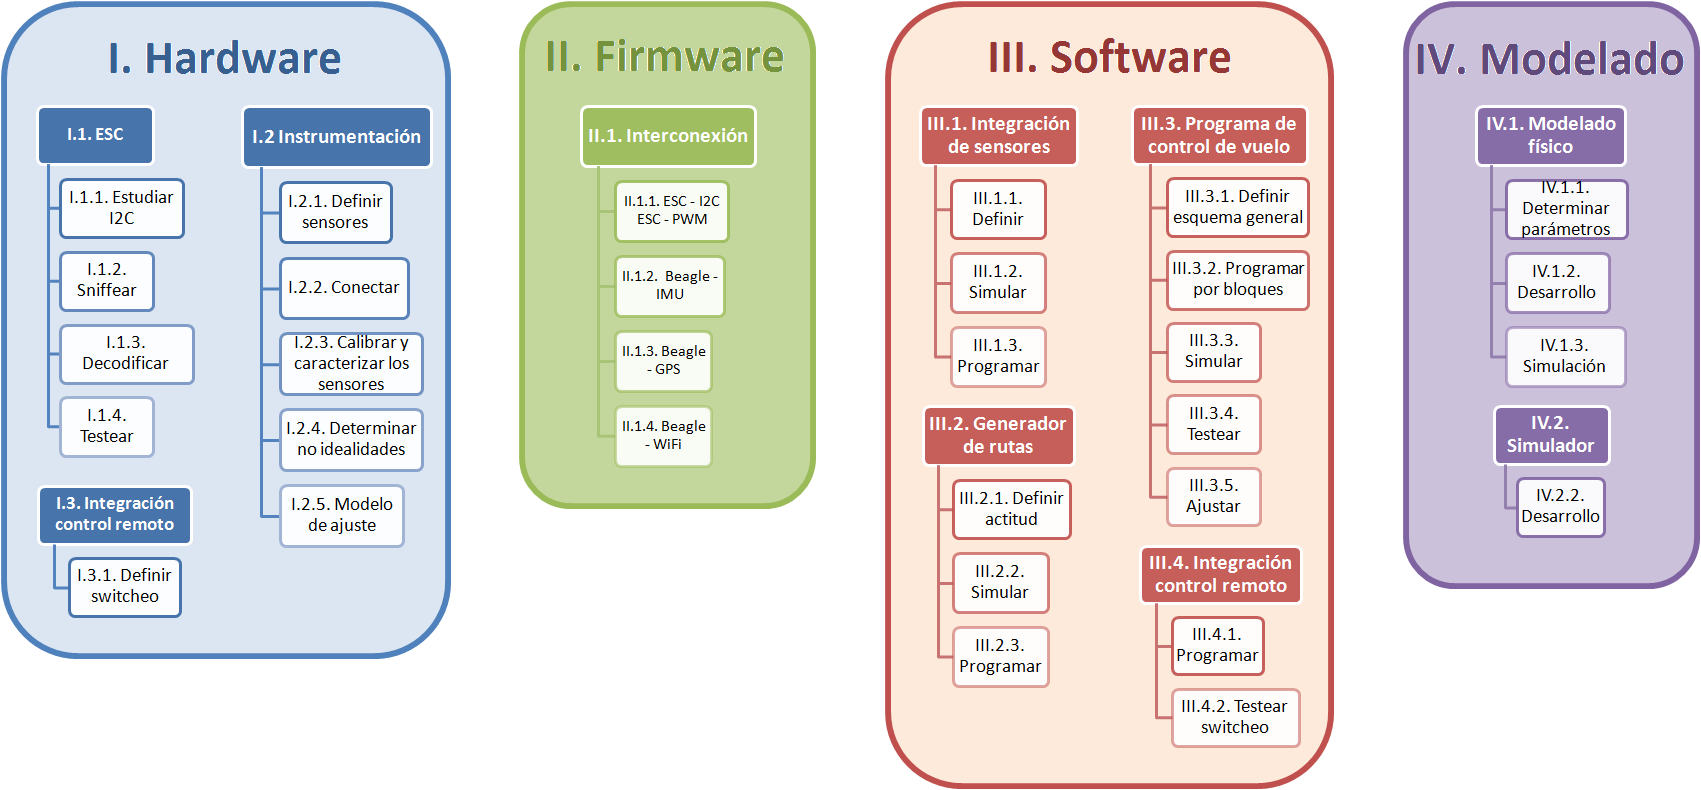
\includegraphics[width=1\textwidth]{./division.png}
	\caption{División de tareas}
	\label{fig:div}
\end{figure}

%\begin{enumerate}
%	\item Hacer funcionar el analizador lógico
%	\item Decodificar el código I2C, entenderlo y aprender a enviar comandos
%	\item Probar si los comandos enviados producen el efecto deseado sobre los motores
%	\item Investigar en papers u otros documentos si será necesario incluir algún otro sensor
%	\item Interconectar todos los sensores, armar los conversores de niveles lógicos necesarios
%	\item Investigar e implementar alguna manera de mejorar la presición del GPS
%	\item Definir la forma de realizar el switcheo entre el control remoto y el control automático. Definir el hardware necesario para ello
%	\item Programar el firmware necesario para una buena comunicación entre los \textbf{ESC's} y los motores, ya sea mediante protocolo \textbf{I2C} o \textbf{PWM}
%	\item Programar el firmware necesario para una buena comunicación entre la \textbf{BeagleBoard} y la \textbf{IMU}.
%	\item Programar el firmware necesario para una buena comunicación entre la \textbf{BeagleBoard} y el \textbf{GPS}.
%	\item Programar el firmware necesario para una buena comunicación entre la \textbf{BeagleBoard} y el dispositivo \textbf{Wi-Fi}.
%	\item Definir criterios para integrar los sensores: algoritmo base, interrogación periódica a los sensores, cada cuanto tiempo, en que orden, etc.
%	\item Simular los algoritmos y corroborar el buen funcionamiento teórico.
%	\item Programar los algoritmos definitivos y probarlos
%	\item Definir la actitud de vuelo del cuadricóptero.
%	\item simular vuelo en MatLab.
%	\item Programar algoritmos definitivos y testearlos.
%	\item Definir el esquema general de los algoritmos de control
%	\item Programar los distintos bloques de control y su interrelación
%	\item Simular algoritmos de control
%	\item Testear algoritmos de control
%	\item Realizar los ajustes necesarios y reprogramar si es necesario
%	\item Programar el software necesario para la conmutación entre el control automático y el remoto.
%	\item Testear el switcheo del mando automático al manual y realizar los ajustes necesarios.
%	\item Desarrollo del modelo físico y contrastación con papers existentes
%	\item Simular el comportamiento del cuadricóptero según el modelo físico.
%	\item Desarrollar el simulador en MatLab
%	\item Identificar las no idealidades de los sensores
%	\item Implementar un modelo de ajuste de las medidas tomadas por los sensores, diseñar pruebas y en función de estas hallar los parámetros de los modelos propuestos para finalmente calibrar de la mejor forma los sensores.
%\end{enumerate}

\begin{table}[H]
\begin{tabular}{|p{50pt}|p{220pt}|p{60pt}|p{20pt}|p{20pt}|} 
\hline
\cellcolor[gray]{0.8} $N^o$ \textbf{tarea} & \cellcolor[gray]{0.8} \textbf{Descripción} & \cellcolor[gray]{0.8} \textbf{Recursos} & \cellcolor[gray]{0.8} \textbf{T1} & \cellcolor[gray]{0.8} \textbf{T2} \\ \hline
I.1.1  & Buscar implementaciones del protocolo I2C, entenderlo y estudiar su funcionamiento & TODOS & 7 & 10\\ \hline
I.1.2  & Hacer funcionar el analizador lógico y aprender a utilizar el software correspondiente. & M. L. & 7 & 14\\ \hline
I.1.3  & Diseñar pruebas para la caracterización de los ESCs, decodificar el código I2C, entenderlo y aprender a enviar comandos & M. L., M. T. & 7 & 14\\ \hline
I.1.4  & Probar si los comandos enviados producen el efecto deseado sobre los motores. Para ello se deberá caracterizar los motores y las relaciones código $i^2c$ - velocidad de giro y código $i^2c$ - fuerza & M.T., S.P. & 20 & 30\\ \hline
I.2.1  & Investigar en papers u otros documentos si será necesario incluir algún otro sensor & TODOS & 5 & 7 \\ \hline
\end{tabular}
\end{table}
\begin{table}[H]
\begin{tabular}{|p{50pt}|p{220pt}|p{60pt}|p{20pt}|p{20pt}|} 
\hline
I.2.2  & Conectar todos los sensores, armar los conversores de niveles lógicos necesarios & M. T. & 2 & 5 \\ \hline

I.2.3  & Diseñar pruebas y en función de estas calibrar de la mejor forma posible los sensores. Investigar e implementar alguna manera de mejorar la precisión de los sensores  & S. P., M. T. & 14 & 25 \\ \hline
I.2.4 & Identificar las no idealidades de los sensores & S. P., M. T. & 14 & 25 \\ \hline
I.2.5 & Implementar un modelo de ajuste de las medidas tomadas por los sensores & S. P., M. T. & 3 & 5 \\ \hline
I.3.1 & Definir la forma de realizar el switcheo entre el control remoto y el control automático. Definir el hardware necesario para ello & TODOS  & 1 & 2\\ \hline \hline
II.1.1  & Programar el firmware necesario para una buena comunicación entre los \textbf{ESC's} y los motores, ya sea mediante protocolo \textbf{I2C} o \textbf{PWM} & M. L. & 7 & 10 \\ \hline
II.1.2  & Programar el firmware necesario para una buena comunicación entre la \textbf{BeagleBoard} y la \textbf{IMU}. & R. R. & 7 & 14 \\ \hline
II.1.3  & Programar el firmware necesario para una buena comunicación entre la \textbf{BeagleBoard} y el \textbf{GPS}. & R. .R  & 4 & 7\\ \hline 
II.1.4  & Programar el firmware necesario para una buena comunicación entre la \textbf{BeagleBoard} y el dispositivo \textbf{Wi-Fi}. & M. T. & 7 & 14 \\ \hline \hline
III.1.1  & Definir criterios para integrar los sensores: algoritmo base, interrogación periódica a los sensores, cada cuanto tiempo, en que orden, etc. & S. P., R. R. & 2 & 5 \\ \hline
III.1.2  & Simular los algoritmos y corroborar el buen funcionamiento teórico. & S. P., R. R.  & 7 & 14\\ \hline
III.1.3  & Programar los algoritmos definitivos y probarlos & S. P., R. R.  & 5 & 10\\ \hline 
III.2.1  & Definir la actitud de vuelo del cuadricóptero. & TODOS  & 1 & 3\\ \hline
III.2.2  & Simular vuelo en MatLab. & M. T. & 5 & 10 \\ \hline
III.2.3  & Programar algoritmos definitivos y testearlos. & R. R. & 7 & 14 \\ \hline
III.3.1  & Definir el esquema general de los algoritmos de control & TODOS & 2 & 5 \\ \hline
III.3.2  & Programar los distintos bloques de control y su interrelación & TODOS & 14 & 20 \\ \hline
III.3.3  & Simular algoritmos de control & TODOS  & 5 & 7\\ \hline
III.3.4  & Testear algoritmos de control & TODOS  & 20 & 30\\ \hline
\end{tabular}
\end{table}
\begin{table}[H]
\begin{tabular}{|p{50pt}|p{220pt}|p{60pt}|p{20pt}|p{20pt}|} 
\hline
III.3.5  & Realizar los ajustes necesarios y reprogramar si es necesario & TODOS  & 20 & 30\\ \hline
III.4.1  & Programar el software necesario para la conmutación entre el control automático y el remoto. & TODOS  & 14 & 20 \\ \hline
III.4.2  & Testear el switcheo del mando automático al manual y realizar los ajustes necesarios. & TODOS & 14 & 20 \\ \hline \hline
IV.1.1  &  Determinar los parámetros del cuadricóptero con la mayor exactitud posible, como pueden ser la masa o el tamaño.  &  M.L. & 1 & 2\\ \hline
IV.1.2  & Desarrollo del modelo físico y contrastación con papers existentes & S. P. & 7 & 14 \\ \hline
IV.1.3  &  Simular el comportamiento del cuadricóptero según el modelo físico. & S. P.  & 7 & 14  \\ \hline
IV.2.2  &  Desarrollar el simulador en MatLab & S. P., M. T.  & 20 & 30 \\ \hline
\end{tabular} 
\caption{Descripción de las tareas y asignación de recursos}
\label{tab:tareas_y_recursos}
\end{table}

\end{document}